\documentclass[1p]{elsarticle_modified}
%\bibliographystyle{elsarticle-num}

%\usepackage[colorlinks]{hyperref}
%\usepackage{abbrmath_seonhwa} %\Abb, \Ascr, \Acal ,\Abf, \Afrak
\usepackage{amsfonts}
\usepackage{amssymb}
\usepackage{amsmath}
\usepackage{amsthm}
\usepackage{scalefnt}
\usepackage{amsbsy}
\usepackage{kotex}
\usepackage{caption}
\usepackage{subfig}
\usepackage{color}
\usepackage{graphicx}
\usepackage{xcolor} %% white, black, red, green, blue, cyan, magenta, yellow
\usepackage{float}
\usepackage{setspace}
\usepackage{hyperref}

\usepackage{tikz}
\usetikzlibrary{arrows}

\usepackage{multirow}
\usepackage{array} % fixed length table
\usepackage{hhline}

%%%%%%%%%%%%%%%%%%%%%
\makeatletter
\renewcommand*\env@matrix[1][\arraystretch]{%
	\edef\arraystretch{#1}%
	\hskip -\arraycolsep
	\let\@ifnextchar\new@ifnextchar
	\array{*\c@MaxMatrixCols c}}
\makeatother %https://tex.stackexchange.com/questions/14071/how-can-i-increase-the-line-spacing-in-a-matrix
%%%%%%%%%%%%%%%

\usepackage[normalem]{ulem}

\newcommand{\msout}[1]{\ifmmode\text{\sout{\ensuremath{#1}}}\else\sout{#1}\fi}
%SOURCE: \msout is \stkout macro in https://tex.stackexchange.com/questions/20609/strikeout-in-math-mode

\newcommand{\cancel}[1]{
	\ifmmode
	{\color{red}\msout{#1}}
	\else
	{\color{red}\sout{#1}}
	\fi
}

\newcommand{\add}[1]{
	{\color{blue}\uwave{#1}}
}

\newcommand{\replace}[2]{
	\ifmmode
	{\color{red}\msout{#1}}{\color{blue}\uwave{#2}}
	\else
	{\color{red}\sout{#1}}{\color{blue}\uwave{#2}}
	\fi
}

\newcommand{\Sol}{\mathcal{S}} %segment
\newcommand{\D}{D} %diagram
\newcommand{\A}{\mathcal{A}} %arc


%%%%%%%%%%%%%%%%%%%%%%%%%%%%%5 test

\def\sl{\operatorname{\textup{SL}}(2,\Cbb)}
\def\psl{\operatorname{\textup{PSL}}(2,\Cbb)}
\def\quan{\mkern 1mu \triangleright \mkern 1mu}

\theoremstyle{definition}
\newtheorem{thm}{Theorem}[section]
\newtheorem{prop}[thm]{Proposition}
\newtheorem{lem}[thm]{Lemma}
\newtheorem{ques}[thm]{Question}
\newtheorem{cor}[thm]{Corollary}
\newtheorem{defn}[thm]{Definition}
\newtheorem{exam}[thm]{Example}
\newtheorem{rmk}[thm]{Remark}
\newtheorem{alg}[thm]{Algorithm}

\newcommand{\I}{\sqrt{-1}}
\begin{document}

%\begin{frontmatter}
%
%\title{Boundary parabolic representations of knots up to 8 crossings}
%
%%% Group authors per affiliation:
%\author{Yunhi Cho} 
%\address{Department of Mathematics, University of Seoul, Seoul, Korea}
%\ead{yhcho@uos.ac.kr}
%
%
%\author{Seonhwa Kim} %\fnref{s_kim}}
%\address{Center for Geometry and Physics, Institute for Basic Science, Pohang, 37673, Korea}
%\ead{ryeona17@ibs.re.kr}
%
%\author{Hyuk Kim}
%\address{Department of Mathematical Sciences, Seoul National University, Seoul 08826, Korea}
%\ead{hyukkim@snu.ac.kr}
%
%\author{Seokbeom Yoon}
%\address{Department of Mathematical Sciences, Seoul National University, Seoul, 08826,  Korea}
%\ead{sbyoon15@snu.ac.kr}
%
%\begin{abstract}
%We find all boundary parabolic representation of knots up to 8 crossings.
%
%\end{abstract}
%\begin{keyword}
%    \MSC[2010] 57M25 
%\end{keyword}
%
%\end{frontmatter}

%\linenumbers
%\tableofcontents
%
\newcommand\colored[1]{\textcolor{white}{\rule[-0.35ex]{0.8em}{1.4ex}}\kern-0.8em\color{red} #1}%
%\newcommand\colored[1]{\textcolor{white}{ #1}\kern-2.17ex	\textcolor{white}{ #1}\kern-1.81ex	\textcolor{white}{ #1}\kern-2.15ex\color{red}#1	}

{\Large $\underline{11a_{348}~(K11a_{348})}$}

\setlength{\tabcolsep}{10pt}
\renewcommand{\arraystretch}{1.6}
\vspace{1cm}\begin{tabular}{m{100pt}>{\centering\arraybackslash}m{274pt}}
\multirow{5}{120pt}{
	\centering
	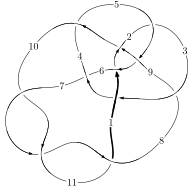
\includegraphics[width=112pt]{../../../GIT/diagram.site/Diagrams/png/597_11a_348.png}\\
\ \ \ A knot diagram\footnotemark}&
\allowdisplaybreaks
\textbf{Linearized knot diagam} \\
\cline{2-2}
 &
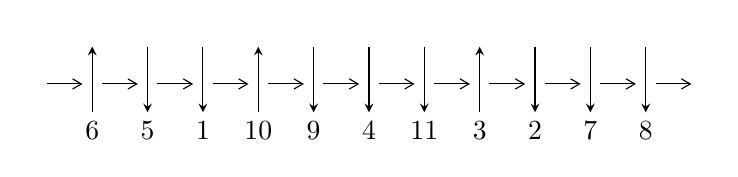
\begin{tikzpicture}[x=20pt, y=17pt]
	% nodes
	\node (C0) at (0, 0) {};
	\node (C1) at (1, 0) {};
	\node (C1U) at (1, +1) {};
	\node (C1D) at (1, -1) {6};

	\node (C2) at (2, 0) {};
	\node (C2U) at (2, +1) {};
	\node (C2D) at (2, -1) {5};

	\node (C3) at (3, 0) {};
	\node (C3U) at (3, +1) {};
	\node (C3D) at (3, -1) {1};

	\node (C4) at (4, 0) {};
	\node (C4U) at (4, +1) {};
	\node (C4D) at (4, -1) {10};

	\node (C5) at (5, 0) {};
	\node (C5U) at (5, +1) {};
	\node (C5D) at (5, -1) {9};

	\node (C6) at (6, 0) {};
	\node (C6U) at (6, +1) {};
	\node (C6D) at (6, -1) {4};

	\node (C7) at (7, 0) {};
	\node (C7U) at (7, +1) {};
	\node (C7D) at (7, -1) {11};

	\node (C8) at (8, 0) {};
	\node (C8U) at (8, +1) {};
	\node (C8D) at (8, -1) {3};

	\node (C9) at (9, 0) {};
	\node (C9U) at (9, +1) {};
	\node (C9D) at (9, -1) {2};

	\node (C10) at (10, 0) {};
	\node (C10U) at (10, +1) {};
	\node (C10D) at (10, -1) {7};

	\node (C11) at (11, 0) {};
	\node (C11U) at (11, +1) {};
	\node (C11D) at (11, -1) {8};
	\node (C12) at (12, 0) {};

	% arrows
	\draw[->,>={angle 60}]
	(C0) edge (C1) (C1) edge (C2) (C2) edge (C3) (C3) edge (C4) (C4) edge (C5) (C5) edge (C6) (C6) edge (C7) (C7) edge (C8) (C8) edge (C9) (C9) edge (C10) (C10) edge (C11) (C11) edge (C12) ;	\draw[->,>=stealth]
	(C1D) edge (C1U) (C2U) edge (C2D) (C3U) edge (C3D) (C4D) edge (C4U) (C5U) edge (C5D) (C6U) edge (C6D) (C7U) edge (C7D) (C8D) edge (C8U) (C9U) edge (C9D) (C10U) edge (C10D) (C11U) edge (C11D) ;
	\end{tikzpicture} \\
\hhline{~~} \\& 
\textbf{Solving Sequence} \\ \cline{2-2} 
 &
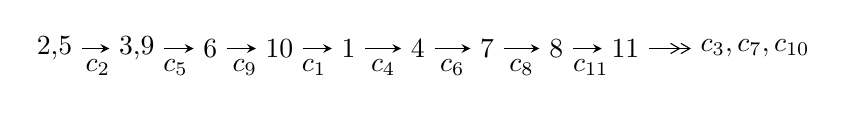
\begin{tikzpicture}[x=25pt, y=7pt]
	% node
	\node (A0) at (-1/8, 0) {2,5};
	\node (A1) at (17/16, 0) {3,9};
	\node (A2) at (17/8, 0) {6};
	\node (A3) at (25/8, 0) {10};
	\node (A4) at (33/8, 0) {1};
	\node (A5) at (41/8, 0) {4};
	\node (A6) at (49/8, 0) {7};
	\node (A7) at (57/8, 0) {8};
	\node (A8) at (65/8, 0) {11};
	\node (C1) at (1/2, -1) {$c_{2}$};
	\node (C2) at (13/8, -1) {$c_{5}$};
	\node (C3) at (21/8, -1) {$c_{9}$};
	\node (C4) at (29/8, -1) {$c_{1}$};
	\node (C5) at (37/8, -1) {$c_{4}$};
	\node (C6) at (45/8, -1) {$c_{6}$};
	\node (C7) at (53/8, -1) {$c_{8}$};
	\node (C8) at (61/8, -1) {$c_{11}$};
	\node (A9) at (10, 0) {$c_{3},c_{7},c_{10}$};

	% edge
	\draw[->,>=stealth]	
	(A0) edge (A1) (A1) edge (A2) (A2) edge (A3) (A3) edge (A4) (A4) edge (A5) (A5) edge (A6) (A6) edge (A7) (A7) edge (A8) ;
	\draw[->>,>={angle 60}]	
	(A8) edge (A9);
\end{tikzpicture} \\ 

\end{tabular} \\

\footnotetext{
The image of knot diagram is generated by the software ``\textbf{Draw programme}" developed by Andrew Bartholomew(\url{http://www.layer8.co.uk/maths/draw/index.htm\#Running-draw}), where we modified some parts for our purpose(\url{https://github.com/CATsTAILs/LinksPainter}).
}\phantom \\ \newline 
\centering \textbf{Ideals for irreducible components\footnotemark of $X_{\text{par}}$} 
 
\begin{align*}
I^u_{1}&=\langle 
-1.83178\times10^{30} u^{28}-4.25498\times10^{31} u^{27}+\cdots+1.83797\times10^{31} b-2.13808\times10^{31},\\
\phantom{I^u_{1}}&\phantom{= \langle  }-2.13808\times10^{31} u^{28}-4.00799\times10^{32} u^{27}+\cdots+1.34172\times10^{33} a+1.06235\times10^{34},\\
\phantom{I^u_{1}}&\phantom{= \langle  }u^{29}+25 u^{28}+\cdots+638 u+73\rangle \\
I^u_{2}&=\langle 
-600 u^{14} a^3-936 u^{14} a^2+\cdots-1792 a-1217,\;8 u^{14} a^3+72 u^{14} a^2+\cdots+218 a+237,\\
\phantom{I^u_{2}}&\phantom{= \langle  }u^{15}-7 u^{14}+23 u^{13}-42 u^{12}+38 u^{11}+7 u^{10}-61 u^9+62 u^8-2 u^7-50 u^6+38 u^5+4 u^4-20 u^3+7 u^2+3 u-2\rangle \\
I^u_{3}&=\langle 
-231789 u^{14}+1842380 u^{13}+\cdots+808985 b-1813670,\\
\phantom{I^u_{3}}&\phantom{= \langle  }-362734 u^{14}+2468395 u^{13}+\cdots+4044925 a+9070125,\;u^{15}-10 u^{14}+\cdots+105 u-25\rangle \\
\\
I^v_{1}&=\langle 
a,\;b^2- b v+2 b- v+3,\;v^2-3 v+1\rangle \\
I^v_{2}&=\langle 
a,\;b^2+b+1,\;v-1\rangle \\
\end{align*}
\raggedright * 5 irreducible components of $\dim_{\mathbb{C}}=0$, with total 110 representations.\\
\footnotetext{All coefficients of polynomials are rational numbers. But the coefficients are sometimes approximated in decimal forms when there is not enough margin.}
\newpage
\renewcommand{\arraystretch}{1}
\centering \section*{I. $I^u_{1}= \langle -1.83\times10^{30} u^{28}-4.25\times10^{31} u^{27}+\cdots+1.84\times10^{31} b-2.14\times10^{31},\;-2.14\times10^{31} u^{28}-4.01\times10^{32} u^{27}+\cdots+1.34\times10^{33} a+1.06\times10^{34},\;u^{29}+25 u^{28}+\cdots+638 u+73 \rangle$}
\flushleft \textbf{(i) Arc colorings}\\
\begin{tabular}{m{7pt} m{180pt} m{7pt} m{180pt} }
\flushright $a_{2}=$&$\begin{pmatrix}1\\0\end{pmatrix}$ \\
\flushright $a_{5}=$&$\begin{pmatrix}0\\u\end{pmatrix}$ \\
\flushright $a_{3}=$&$\begin{pmatrix}1\\u^2\end{pmatrix}$ \\
\flushright $a_{9}=$&$\begin{pmatrix}0.0159354 u^{28}+0.298722 u^{27}+\cdots-40.6500 u-7.91783\\0.0996632 u^{28}+2.31505 u^{27}+\cdots+18.0846 u+1.16328\end{pmatrix}$ \\
\flushright $a_{6}=$&$\begin{pmatrix}0.0368204 u^{28}+0.942895 u^{27}+\cdots+43.0059 u+7.47915\\-0.0223856 u^{28}-0.491135 u^{27}+\cdots+17.0122 u+2.68789\end{pmatrix}$ \\
\flushright $a_{10}=$&$\begin{pmatrix}-0.0837278 u^{28}-2.01633 u^{27}+\cdots-58.7346 u-9.08111\\0.0996632 u^{28}+2.31505 u^{27}+\cdots+18.0846 u+1.16328\end{pmatrix}$ \\
\flushright $a_{1}=$&$\begin{pmatrix}-0.107125 u^{28}-2.64363 u^{27}+\cdots-54.0442 u-5.41609\\0.0340032 u^{28}+0.644747 u^{27}+\cdots-44.9598 u-6.18598\end{pmatrix}$ \\
\flushright $a_{4}=$&$\begin{pmatrix}0.0130859 u^{28}+0.295275 u^{27}+\cdots-5.98849 u+0.469224\\0.0461201 u^{28}+1.13875 u^{27}+\cdots+33.9822 u+4.32204\end{pmatrix}$ \\
\flushright $a_{7}=$&$\begin{pmatrix}0.0636554 u^{28}+1.58804 u^{27}+\cdots+66.1229 u+10.2269\\0.0414256 u^{28}+1.05896 u^{27}+\cdots+53.1661 u+7.35249\end{pmatrix}$ \\
\flushright $a_{8}=$&$\begin{pmatrix}0.0928024 u^{28}+2.19118 u^{27}+\cdots+3.68727 u-1.80570\\-0.0384173 u^{28}-0.676173 u^{27}+\cdots+31.1112 u+3.29583\end{pmatrix}$ \\
\flushright $a_{11}=$&$\begin{pmatrix}-0.0973760 u^{28}-2.33888 u^{27}+\cdots-49.8137 u-6.44579\\-0.0796577 u^{28}-2.01645 u^{27}+\cdots-84.2207 u-11.6200\end{pmatrix}$\\ \flushright $a_{11}=$&$\begin{pmatrix}-0.0973760 u^{28}-2.33888 u^{27}+\cdots-49.8137 u-6.44579\\-0.0796577 u^{28}-2.01645 u^{27}+\cdots-84.2207 u-11.6200\end{pmatrix}$\\&\end{tabular}
\flushleft \textbf{(ii) Obstruction class $= -1$}\\~\\
\flushleft \textbf{(iii) Cusp Shapes $= 0.174043 u^{28}+3.67857 u^{27}+\cdots-96.9970 u-20.7731$}\\~\\
\newpage\renewcommand{\arraystretch}{1}
\flushleft \textbf{(iv) u-Polynomials at the component}\newline \\
\begin{tabular}{m{50pt}|m{274pt}}
Crossings & \hspace{64pt}u-Polynomials at each crossing \\
\hline $$\begin{aligned}c_{1}\end{aligned}$$&$\begin{aligned}
&u^{29}-29 u^{28}+\cdots-131072 u+16384
\end{aligned}$\\
\hline $$\begin{aligned}c_{2}\end{aligned}$$&$\begin{aligned}
&u^{29}-25 u^{28}+\cdots+638 u-73
\end{aligned}$\\
\hline $$\begin{aligned}c_{3},c_{6}\end{aligned}$$&$\begin{aligned}
&u^{29}- u^{28}+\cdots+17 u+1
\end{aligned}$\\
\hline $$\begin{aligned}c_{4},c_{8}\end{aligned}$$&$\begin{aligned}
&u^{29}- u^{28}+\cdots+21 u+9
\end{aligned}$\\
\hline $$\begin{aligned}c_{5},c_{9}\end{aligned}$$&$\begin{aligned}
&u^{29}+2 u^{27}+\cdots+u+1
\end{aligned}$\\
\hline $$\begin{aligned}c_{7},c_{10},c_{11}\end{aligned}$$&$\begin{aligned}
&u^{29}+9 u^{28}+\cdots+49 u+73
\end{aligned}$\\
\hline
\end{tabular}\\~\\
\newpage\renewcommand{\arraystretch}{1}
\flushleft \textbf{(v) Riley Polynomials at the component}\newline \\
\begin{tabular}{m{50pt}|m{274pt}}
Crossings & \hspace{64pt}Riley Polynomials at each crossing \\
\hline $$\begin{aligned}c_{1}\end{aligned}$$&$\begin{aligned}
&y^{29}-7 y^{28}+\cdots+5100273664 y-268435456
\end{aligned}$\\
\hline $$\begin{aligned}c_{2}\end{aligned}$$&$\begin{aligned}
&y^{29}-13 y^{28}+\cdots+27006 y-5329
\end{aligned}$\\
\hline $$\begin{aligned}c_{3},c_{6}\end{aligned}$$&$\begin{aligned}
&y^{29}-7 y^{28}+\cdots+235 y-1
\end{aligned}$\\
\hline $$\begin{aligned}c_{4},c_{8}\end{aligned}$$&$\begin{aligned}
&y^{29}+17 y^{28}+\cdots-225 y-81
\end{aligned}$\\
\hline $$\begin{aligned}c_{5},c_{9}\end{aligned}$$&$\begin{aligned}
&y^{29}+4 y^{28}+\cdots-3 y-1
\end{aligned}$\\
\hline $$\begin{aligned}c_{7},c_{10},c_{11}\end{aligned}$$&$\begin{aligned}
&y^{29}-31 y^{28}+\cdots-8987 y-5329
\end{aligned}$\\
\hline
\end{tabular}\\~\\
\newpage\flushleft \textbf{(vi) Complex Volumes and Cusp Shapes}
$$\begin{array}{c|c|c}  
\text{Solutions to }I^u_{1}& \I (\text{vol} + \sqrt{-1}CS) & \text{Cusp shape}\\
 \hline 
\begin{aligned}
u &= -0.533215 + 0.743878 I \\
a &= \phantom{-}1.068930 - 0.077579 I \\
b &= \phantom{-}0.512259 - 0.836519 I\end{aligned}
 & \phantom{-}2.89664 + 0.46546 I & \phantom{-}1.68040 + 0.26806 I \\ \hline\begin{aligned}
u &= -0.533215 - 0.743878 I \\
a &= \phantom{-}1.068930 + 0.077579 I \\
b &= \phantom{-}0.512259 + 0.836519 I\end{aligned}
 & \phantom{-}2.89664 - 0.46546 I & \phantom{-}1.68040 - 0.26806 I \\ \hline\begin{aligned}
u &= -0.174221 + 0.891733 I \\
a &= -1.045550 - 0.239887 I \\
b &= -0.396072 + 0.890557 I\end{aligned}
 & -2.36877 - 2.03117 I & -4.15870 + 1.99602 I \\ \hline\begin{aligned}
u &= -0.174221 - 0.891733 I \\
a &= -1.045550 + 0.239887 I \\
b &= -0.396072 - 0.890557 I\end{aligned}
 & -2.36877 + 2.03117 I & -4.15870 - 1.99602 I \\ \hline\begin{aligned}
u &= -0.993675 + 0.553218 I \\
a &= -0.840807 + 0.404017 I \\
b &= -0.611979 + 0.866611 I\end{aligned}
 & \phantom{-}1.00519 + 4.10843 I & -1.11851 - 6.27833 I \\ \hline\begin{aligned}
u &= -0.993675 - 0.553218 I \\
a &= -0.840807 - 0.404017 I \\
b &= -0.611979 - 0.866611 I\end{aligned}
 & \phantom{-}1.00519 - 4.10843 I & -1.11851 + 6.27833 I \\ \hline\begin{aligned}
u &= \phantom{-}0.377713 + 0.751230 I \\
a &= \phantom{-}0.598055 + 0.080621 I \\
b &= -0.165328 - 0.479728 I\end{aligned}
 & -0.38938 - 1.51803 I & -2.55495 + 5.06805 I \\ \hline\begin{aligned}
u &= \phantom{-}0.377713 - 0.751230 I \\
a &= \phantom{-}0.598055 - 0.080621 I \\
b &= -0.165328 + 0.479728 I\end{aligned}
 & -0.38938 + 1.51803 I & -2.55495 - 5.06805 I \\ \hline\begin{aligned}
u &= -1.23159 + 0.78729 I \\
a &= -1.036980 + 0.164410 I \\
b &= -1.14770 + 1.01889 I\end{aligned}
 & -4.12024 + 7.78492 I & \phantom{-0.000000 } 0. - 5.99189 I \\ \hline\begin{aligned}
u &= -1.23159 - 0.78729 I \\
a &= -1.036980 - 0.164410 I \\
b &= -1.14770 - 1.01889 I\end{aligned}
 & -4.12024 - 7.78492 I & \phantom{-0.000000 -}0. + 5.99189 I\\
 \hline 
 \end{array}$$\newpage$$\begin{array}{c|c|c}  
\text{Solutions to }I^u_{1}& \I (\text{vol} + \sqrt{-1}CS) & \text{Cusp shape}\\
 \hline 
\begin{aligned}
u &= -1.40924 + 0.62053 I \\
a &= \phantom{-}0.902693 - 0.279351 I \\
b &= \phantom{-}1.09876 - 0.95382 I\end{aligned}
 & -11.42010 + 3.19049 I & \phantom{-0.000000 } 0 \\ \hline\begin{aligned}
u &= -1.40924 - 0.62053 I \\
a &= \phantom{-}0.902693 + 0.279351 I \\
b &= \phantom{-}1.09876 + 0.95382 I\end{aligned}
 & -11.42010 - 3.19049 I & \phantom{-0.000000 } 0 \\ \hline\begin{aligned}
u &= \phantom{-}0.405846 + 0.192100 I \\
a &= -1.56669 - 1.76693 I \\
b &= \phantom{-}0.296405 + 1.018060 I\end{aligned}
 & -5.03403 - 2.22778 I & -7.47163 + 3.53534 I \\ \hline\begin{aligned}
u &= \phantom{-}0.405846 - 0.192100 I \\
a &= -1.56669 + 1.76693 I \\
b &= \phantom{-}0.296405 - 1.018060 I\end{aligned}
 & -5.03403 + 2.22778 I & -7.47163 - 3.53534 I \\ \hline\begin{aligned}
u &= -1.22083 + 0.96772 I \\
a &= \phantom{-}1.004960 - 0.047355 I \\
b &= \phantom{-}1.18107 - 1.03033 I\end{aligned}
 & -4.3561 + 13.4943 I & \phantom{-0.000000 } 0 \\ \hline\begin{aligned}
u &= -1.22083 - 0.96772 I \\
a &= \phantom{-}1.004960 + 0.047355 I \\
b &= \phantom{-}1.18107 + 1.03033 I\end{aligned}
 & -4.3561 - 13.4943 I & \phantom{-0.000000 } 0 \\ \hline\begin{aligned}
u &= \phantom{-}0.009310 + 0.427042 I \\
a &= \phantom{-}2.26846 + 1.69136 I \\
b &= \phantom{-}0.701162 - 0.984473 I\end{aligned}
 & -4.65620 + 1.98203 I & -8.58633 - 3.04801 I \\ \hline\begin{aligned}
u &= \phantom{-}0.009310 - 0.427042 I \\
a &= \phantom{-}2.26846 - 1.69136 I \\
b &= \phantom{-}0.701162 + 0.984473 I\end{aligned}
 & -4.65620 - 1.98203 I & -8.58633 + 3.04801 I \\ \hline\begin{aligned}
u &= -1.27872 + 1.09142 I \\
a &= -0.946459 + 0.001404 I \\
b &= -1.20873 + 1.03478 I\end{aligned}
 & -11.5069 + 17.5600 I & \phantom{-0.000000 } 0 \\ \hline\begin{aligned}
u &= -1.27872 - 1.09142 I \\
a &= -0.946459 - 0.001404 I \\
b &= -1.20873 - 1.03478 I\end{aligned}
 & -11.5069 - 17.5600 I & \phantom{-0.000000 } 0\\
 \hline 
 \end{array}$$\newpage$$\begin{array}{c|c|c}  
\text{Solutions to }I^u_{1}& \I (\text{vol} + \sqrt{-1}CS) & \text{Cusp shape}\\
 \hline 
\begin{aligned}
u &= -0.290088\phantom{ +0.000000I} \\
a &= -2.49108\phantom{ +0.000000I} \\
b &= -0.722632\phantom{ +0.000000I}\end{aligned}
 & -1.41973\phantom{ +0.000000I} & -5.24450\phantom{ +0.000000I} \\ \hline\begin{aligned}
u &= -1.84285 + 0.37896 I \\
a &= -0.221920 + 0.459486 I \\
b &= -0.234839 + 0.930861 I\end{aligned}
 & -0.10408 + 3.63440 I & \phantom{-0.000000 } 0 \\ \hline\begin{aligned}
u &= -1.84285 - 0.37896 I \\
a &= -0.221920 - 0.459486 I \\
b &= -0.234839 - 0.930861 I\end{aligned}
 & -0.10408 - 3.63440 I & \phantom{-0.000000 } 0 \\ \hline\begin{aligned}
u &= -0.97578 + 1.61172 I \\
a &= \phantom{-}0.037347 + 0.297762 I \\
b &= \phantom{-}0.516352 + 0.230358 I\end{aligned}
 & -2.86261 - 4.93654 I & \phantom{-0.000000 } 0 \\ \hline\begin{aligned}
u &= -0.97578 - 1.61172 I \\
a &= \phantom{-}0.037347 - 0.297762 I \\
b &= \phantom{-}0.516352 - 0.230358 I\end{aligned}
 & -2.86261 + 4.93654 I & \phantom{-0.000000 } 0 \\ \hline\begin{aligned}
u &= -1.81822 + 1.09987 I \\
a &= \phantom{-}0.375121 - 0.181419 I \\
b &= \phantom{-}0.482516 - 0.742445 I\end{aligned}
 & -8.14903 + 8.41158 I & \phantom{-0.000000 } 0 \\ \hline\begin{aligned}
u &= -1.81822 - 1.09987 I \\
a &= \phantom{-}0.375121 + 0.181419 I \\
b &= \phantom{-}0.482516 + 0.742445 I\end{aligned}
 & -8.14903 - 8.41158 I & \phantom{-0.000000 } 0 \\ \hline\begin{aligned}
u &= -1.66948 + 1.64303 I \\
a &= -0.180391 - 0.219962 I \\
b &= -0.662563 - 0.070835 I\end{aligned}
 & -10.73200 - 7.71685 I & \phantom{-0.000000 } 0 \\ \hline\begin{aligned}
u &= -1.66948 - 1.64303 I \\
a &= -0.180391 + 0.219962 I \\
b &= -0.662563 + 0.070835 I\end{aligned}
 & -10.73200 + 7.71685 I & \phantom{-0.000000 } 0\\
 \hline 
 \end{array}$$\newpage\newpage\renewcommand{\arraystretch}{1}
\centering \section*{II. $I^u_{2}= \langle -600 u^{14} a^3-936 u^{14} a^2+\cdots-1792 a-1217,\;8 u^{14} a^3+72 u^{14} a^2+\cdots+218 a+237,\;u^{15}-7 u^{14}+\cdots+3 u-2 \rangle$}
\flushleft \textbf{(i) Arc colorings}\\
\begin{tabular}{m{7pt} m{180pt} m{7pt} m{180pt} }
\flushright $a_{2}=$&$\begin{pmatrix}1\\0\end{pmatrix}$ \\
\flushright $a_{5}=$&$\begin{pmatrix}0\\u\end{pmatrix}$ \\
\flushright $a_{3}=$&$\begin{pmatrix}1\\u^2\end{pmatrix}$ \\
\flushright $a_{9}=$&$\begin{pmatrix}a\\0.669643 a^{3} u^{14}+1.04464 a^{2} u^{14}+\cdots+2 a+1.35826\end{pmatrix}$ \\
\flushright $a_{6}=$&$\begin{pmatrix}- a^2 u\\-1.04464 a^{3} u^{14}-0.669643 a^{2} u^{14}+\cdots+6 a+1.00112\end{pmatrix}$ \\
\flushright $a_{10}=$&$\begin{pmatrix}-0.669643 a^{3} u^{14}-1.04464 a^{2} u^{14}+\cdots-a-1.35826\\0.669643 a^{3} u^{14}+1.04464 a^{2} u^{14}+\cdots+2 a+1.35826\end{pmatrix}$ \\
\flushright $a_{1}=$&$\begin{pmatrix}-0.477679 a^{3} u^{14}+0.334821 a^{2} u^{14}+\cdots-2 a+0.499442\\-1.04464 a^{3} u^{14}-0.669643 a^{2} u^{14}+\cdots+6 a+0.00111607\end{pmatrix}$ \\
\flushright $a_{4}=$&$\begin{pmatrix}0.821429 a^{3} u^{14}+0.321429 a^{2} u^{14}+\cdots-0.678571 a^{2}+0.00446429\\0.223214 a^{3} u^{14}+0.348214 a^{2} u^{14}+\cdots-6 a-1.00558\end{pmatrix}$ \\
\flushright $a_{7}=$&$\begin{pmatrix}0.254464 a^{3} u^{14}+0.316964 a^{2} u^{14}+\cdots-0.683036 a^{2}+0.506138\\-0.866071 a^{3} u^{14}+0.00892857 a^{2} u^{14}+\cdots+2.00893 a^{2}-0.00334821\end{pmatrix}$ \\
\flushright $a_{8}=$&$\begin{pmatrix}-0.669643 a^{3} u^{14}-1.04464 a^{2} u^{14}+\cdots-a-1.35826\\0.991071 a^{3} u^{14}-0.133929 a^{2} u^{14}+\cdots+4 a+1.92522\end{pmatrix}$ \\
\flushright $a_{11}=$&$\begin{pmatrix}-0.254464 a^{3} u^{14}-0.316964 a^{2} u^{14}+\cdots-3 a-0.506138\\-\frac{3}{8} u^{14} a^3+\frac{3}{8} u^{14} a^2+\cdots+6 a+\frac{63}{64}\end{pmatrix}$\\ \flushright $a_{11}=$&$\begin{pmatrix}-0.254464 a^{3} u^{14}-0.316964 a^{2} u^{14}+\cdots-3 a-0.506138\\-\frac{3}{8} u^{14} a^3+\frac{3}{8} u^{14} a^2+\cdots+6 a+\frac{63}{64}\end{pmatrix}$\\&\end{tabular}
\flushleft \textbf{(ii) Obstruction class $= -1$}\\~\\
\flushleft \textbf{(iii) Cusp Shapes $= \frac{117}{28} u^{14} a^3+\frac{75}{28} u^{14} a^2+\cdots-24 a-\frac{7393}{224}$}\\~\\
\newpage\renewcommand{\arraystretch}{1}
\flushleft \textbf{(iv) u-Polynomials at the component}\newline \\
\begin{tabular}{m{50pt}|m{274pt}}
Crossings & \hspace{64pt}u-Polynomials at each crossing \\
\hline $$\begin{aligned}c_{1}\end{aligned}$$&$\begin{aligned}
&(u^2+u+1)^{30}
\end{aligned}$\\
\hline $$\begin{aligned}c_{2}\end{aligned}$$&$\begin{aligned}
&(u^{15}+7 u^{14}+\cdots+3 u+2)^{4}
\end{aligned}$\\
\hline $$\begin{aligned}c_{3},c_{6}\end{aligned}$$&$\begin{aligned}
&u^{60}+3 u^{59}+\cdots+5800 u+1951
\end{aligned}$\\
\hline $$\begin{aligned}c_{4},c_{8}\end{aligned}$$&$\begin{aligned}
&u^{60}+17 u^{58}+\cdots+63147 u+112777
\end{aligned}$\\
\hline $$\begin{aligned}c_{5},c_{9}\end{aligned}$$&$\begin{aligned}
&u^{60}-9 u^{58}+\cdots+5 u+1
\end{aligned}$\\
\hline $$\begin{aligned}c_{7},c_{10},c_{11}\end{aligned}$$&$\begin{aligned}
&(u^{15}-2 u^{14}+\cdots+2 u-1)^{4}
\end{aligned}$\\
\hline
\end{tabular}\\~\\
\newpage\renewcommand{\arraystretch}{1}
\flushleft \textbf{(v) Riley Polynomials at the component}\newline \\
\begin{tabular}{m{50pt}|m{274pt}}
Crossings & \hspace{64pt}Riley Polynomials at each crossing \\
\hline $$\begin{aligned}c_{1}\end{aligned}$$&$\begin{aligned}
&(y^2+y+1)^{30}
\end{aligned}$\\
\hline $$\begin{aligned}c_{2}\end{aligned}$$&$\begin{aligned}
&(y^{15}-3 y^{14}+\cdots+37 y-4)^{4}
\end{aligned}$\\
\hline $$\begin{aligned}c_{3},c_{6}\end{aligned}$$&$\begin{aligned}
&y^{60}-31 y^{59}+\cdots-116686266 y+3806401
\end{aligned}$\\
\hline $$\begin{aligned}c_{4},c_{8}\end{aligned}$$&$\begin{aligned}
&y^{60}+34 y^{59}+\cdots+352063429739 y+12718651729
\end{aligned}$\\
\hline $$\begin{aligned}c_{5},c_{9}\end{aligned}$$&$\begin{aligned}
&y^{60}-18 y^{59}+\cdots+27 y+1
\end{aligned}$\\
\hline $$\begin{aligned}c_{7},c_{10},c_{11}\end{aligned}$$&$\begin{aligned}
&(y^{15}-16 y^{14}+\cdots+10 y-1)^{4}
\end{aligned}$\\
\hline
\end{tabular}\\~\\
\newpage\flushleft \textbf{(vi) Complex Volumes and Cusp Shapes}
$$\begin{array}{c|c|c}  
\text{Solutions to }I^u_{2}& \I (\text{vol} + \sqrt{-1}CS) & \text{Cusp shape}\\
 \hline 
\begin{aligned}
u &= \phantom{-}0.602091 + 0.799295 I \\
a &= \phantom{-}0.967192 + 0.023712 I \\
b &= \phantom{-}1.46023 + 0.91520 I\end{aligned}
 & -0.38534 - 5.63362 I & -2.44329 + 10.98878 I \\ \hline\begin{aligned}
u &= \phantom{-}0.602091 + 0.799295 I \\
a &= \phantom{-}0.731075 + 0.157864 I \\
b &= -0.023707 - 0.161225 I\end{aligned}
 & -0.38534 - 1.57385 I & -2.44329 + 4.06057 I \\ \hline\begin{aligned}
u &= \phantom{-}0.602091 + 0.799295 I \\
a &= -1.60848 + 0.61527 I \\
b &= -0.563384 - 0.787348 I\end{aligned}
 & -0.38534 - 5.63362 I & -2.44329 + 10.98878 I \\ \hline\begin{aligned}
u &= \phantom{-}0.602091 + 0.799295 I \\
a &= \phantom{-}0.142942 + 0.078015 I \\
b &= -0.313994 - 0.679393 I\end{aligned}
 & -0.38534 - 1.57385 I & -2.44329 + 4.06057 I \\ \hline\begin{aligned}
u &= \phantom{-}0.602091 - 0.799295 I \\
a &= \phantom{-}0.967192 - 0.023712 I \\
b &= \phantom{-}1.46023 - 0.91520 I\end{aligned}
 & -0.38534 + 5.63362 I & -2.44329 - 10.98878 I \\ \hline\begin{aligned}
u &= \phantom{-}0.602091 - 0.799295 I \\
a &= \phantom{-}0.731075 - 0.157864 I \\
b &= -0.023707 + 0.161225 I\end{aligned}
 & -0.38534 + 1.57385 I & -2.44329 - 4.06057 I \\ \hline\begin{aligned}
u &= \phantom{-}0.602091 - 0.799295 I \\
a &= -1.60848 - 0.61527 I \\
b &= -0.563384 + 0.787348 I\end{aligned}
 & -0.38534 + 5.63362 I & -2.44329 - 10.98878 I \\ \hline\begin{aligned}
u &= \phantom{-}0.602091 - 0.799295 I \\
a &= \phantom{-}0.142942 - 0.078015 I \\
b &= -0.313994 + 0.679393 I\end{aligned}
 & -0.38534 + 1.57385 I & -2.44329 - 4.06057 I \\ \hline\begin{aligned}
u &= -0.754169 + 0.212783 I \\
a &= -0.910516 + 0.108757 I \\
b &= -1.26285 - 1.50931 I\end{aligned}
 & -10.63760 + 8.63903 I & -15.1406 - 9.1585 I \\ \hline\begin{aligned}
u &= -0.754169 + 0.212783 I \\
a &= \phantom{-}1.194270 + 0.576398 I \\
b &= \phantom{-}1.00815 - 1.23211 I\end{aligned}
 & -10.63760 + 4.57927 I & -15.1406 - 2.2303 I\\
 \hline 
 \end{array}$$\newpage$$\begin{array}{c|c|c}  
\text{Solutions to }I^u_{2}& \I (\text{vol} + \sqrt{-1}CS) & \text{Cusp shape}\\
 \hline 
\begin{aligned}
u &= -0.754169 + 0.212783 I \\
a &= \phantom{-}1.66516 - 1.16392 I \\
b &= \phantom{-}1.023330 + 0.180581 I\end{aligned}
 & -10.63760 + 4.57927 I & -15.1406 - 2.2303 I \\ \hline\begin{aligned}
u &= -0.754169 + 0.212783 I \\
a &= -1.02801 - 2.29134 I \\
b &= -0.663541 + 0.275764 I\end{aligned}
 & -10.63760 + 8.63903 I & -15.1406 - 9.1585 I \\ \hline\begin{aligned}
u &= -0.754169 - 0.212783 I \\
a &= -0.910516 - 0.108757 I \\
b &= -1.26285 + 1.50931 I\end{aligned}
 & -10.63760 - 8.63903 I & -15.1406 + 9.1585 I \\ \hline\begin{aligned}
u &= -0.754169 - 0.212783 I \\
a &= \phantom{-}1.194270 - 0.576398 I \\
b &= \phantom{-}1.00815 + 1.23211 I\end{aligned}
 & -10.63760 - 4.57927 I & -15.1406 + 2.2303 I \\ \hline\begin{aligned}
u &= -0.754169 - 0.212783 I \\
a &= \phantom{-}1.66516 + 1.16392 I \\
b &= \phantom{-}1.023330 - 0.180581 I\end{aligned}
 & -10.63760 - 4.57927 I & -15.1406 + 2.2303 I \\ \hline\begin{aligned}
u &= -0.754169 - 0.212783 I \\
a &= -1.02801 + 2.29134 I \\
b &= -0.663541 - 0.275764 I\end{aligned}
 & -10.63760 - 8.63903 I & -15.1406 + 9.1585 I \\ \hline\begin{aligned}
u &= \phantom{-}0.671611 + 0.294946 I \\
a &= -0.839523 - 0.242865 I \\
b &= -1.36585 - 1.21898 I\end{aligned}
 & -2.26591 - 2.26892 I & -13.6402 + 6.9635 I \\ \hline\begin{aligned}
u &= \phantom{-}0.671611 + 0.294946 I \\
a &= -0.467370 + 0.332502 I \\
b &= -0.67510 + 1.24619 I\end{aligned}
 & -2.26591 + 1.79084 I & -13.64024 + 0.03534 I \\ \hline\begin{aligned}
u &= \phantom{-}0.671611 + 0.294946 I \\
a &= \phantom{-}0.15954 - 1.92560 I \\
b &= \phantom{-}0.411961 - 0.085463 I\end{aligned}
 & -2.26591 + 1.79084 I & -13.64024 + 0.03534 I \\ \hline\begin{aligned}
u &= \phantom{-}0.671611 + 0.294946 I \\
a &= \phantom{-}2.37310 + 0.77283 I \\
b &= \phantom{-}0.492201 + 0.410725 I\end{aligned}
 & -2.26591 - 2.26892 I & -13.6402 + 6.9635 I\\
 \hline 
 \end{array}$$\newpage$$\begin{array}{c|c|c}  
\text{Solutions to }I^u_{2}& \I (\text{vol} + \sqrt{-1}CS) & \text{Cusp shape}\\
 \hline 
\begin{aligned}
u &= \phantom{-}0.671611 - 0.294946 I \\
a &= -0.839523 + 0.242865 I \\
b &= -1.36585 + 1.21898 I\end{aligned}
 & -2.26591 + 2.26892 I & -13.6402 - 6.9635 I \\ \hline\begin{aligned}
u &= \phantom{-}0.671611 - 0.294946 I \\
a &= -0.467370 - 0.332502 I \\
b &= -0.67510 - 1.24619 I\end{aligned}
 & -2.26591 - 1.79084 I & -13.64024 - 0.03534 I \\ \hline\begin{aligned}
u &= \phantom{-}0.671611 - 0.294946 I \\
a &= \phantom{-}0.15954 + 1.92560 I \\
b &= \phantom{-}0.411961 + 0.085463 I\end{aligned}
 & -2.26591 - 1.79084 I & -13.64024 - 0.03534 I \\ \hline\begin{aligned}
u &= \phantom{-}0.671611 - 0.294946 I \\
a &= \phantom{-}2.37310 - 0.77283 I \\
b &= \phantom{-}0.492201 - 0.410725 I\end{aligned}
 & -2.26591 + 2.26892 I & -13.6402 - 6.9635 I \\ \hline\begin{aligned}
u &= \phantom{-}0.581967 + 1.140370 I \\
a &= -0.962013 + 0.055914 I \\
b &= -1.43681 - 0.76472 I\end{aligned}
 & -5.74830 - 8.10302 I & -7.68774 + 10.38587 I \\ \hline\begin{aligned}
u &= \phantom{-}0.581967 + 1.140370 I \\
a &= -0.797951 + 0.360993 I \\
b &= -0.209830 - 0.145532 I\end{aligned}
 & -5.74830 - 4.04325 I & -7.68774 + 3.45767 I \\ \hline\begin{aligned}
u &= \phantom{-}0.581967 + 1.140370 I \\
a &= \phantom{-}1.042160 - 0.728098 I \\
b &= \phantom{-}0.623622 + 1.064510 I\end{aligned}
 & -5.74830 - 8.10302 I & -7.68774 + 10.38587 I \\ \hline\begin{aligned}
u &= \phantom{-}0.581967 + 1.140370 I \\
a &= \phantom{-}0.175748 - 0.094312 I \\
b &= \phantom{-}0.876048 + 0.699876 I\end{aligned}
 & -5.74830 - 4.04325 I & -7.68774 + 3.45767 I \\ \hline\begin{aligned}
u &= \phantom{-}0.581967 - 1.140370 I \\
a &= -0.962013 - 0.055914 I \\
b &= -1.43681 + 0.76472 I\end{aligned}
 & -5.74830 + 8.10302 I & -7.68774 - 10.38587 I \\ \hline\begin{aligned}
u &= \phantom{-}0.581967 - 1.140370 I \\
a &= -0.797951 - 0.360993 I \\
b &= -0.209830 + 0.145532 I\end{aligned}
 & -5.74830 + 4.04325 I & -7.68774 - 3.45767 I\\
 \hline 
 \end{array}$$\newpage$$\begin{array}{c|c|c}  
\text{Solutions to }I^u_{2}& \I (\text{vol} + \sqrt{-1}CS) & \text{Cusp shape}\\
 \hline 
\begin{aligned}
u &= \phantom{-}0.581967 - 1.140370 I \\
a &= \phantom{-}1.042160 + 0.728098 I \\
b &= \phantom{-}0.623622 - 1.064510 I\end{aligned}
 & -5.74830 + 8.10302 I & -7.68774 - 10.38587 I \\ \hline\begin{aligned}
u &= \phantom{-}0.581967 - 1.140370 I \\
a &= \phantom{-}0.175748 + 0.094312 I \\
b &= \phantom{-}0.876048 - 0.699876 I\end{aligned}
 & -5.74830 + 4.04325 I & -7.68774 - 3.45767 I \\ \hline\begin{aligned}
u &= -0.643976 + 0.089739 I \\
a &= \phantom{-}1.093330 - 0.083941 I \\
b &= \phantom{-}1.33517 + 1.40617 I\end{aligned}
 & -3.68331 + 4.69916 I & -15.6538 - 8.3078 I \\ \hline\begin{aligned}
u &= -0.643976 + 0.089739 I \\
a &= -1.303550 - 0.278242 I \\
b &= -1.23743 + 1.19471 I\end{aligned}
 & -3.68331 + 0.63939 I & -15.6538 - 1.3796 I \\ \hline\begin{aligned}
u &= -0.643976 + 0.089739 I \\
a &= -2.13854 + 1.55720 I \\
b &= -0.864422 - 0.062203 I\end{aligned}
 & -3.68331 + 0.63939 I & -15.6538 - 1.3796 I \\ \hline\begin{aligned}
u &= -0.643976 + 0.089739 I \\
a &= \phantom{-}1.73533 + 2.42540 I \\
b &= \phantom{-}0.696542 - 0.152170 I\end{aligned}
 & -3.68331 + 4.69916 I & -15.6538 - 8.3078 I \\ \hline\begin{aligned}
u &= -0.643976 - 0.089739 I \\
a &= \phantom{-}1.093330 + 0.083941 I \\
b &= \phantom{-}1.33517 - 1.40617 I\end{aligned}
 & -3.68331 - 4.69916 I & -15.6538 + 8.3078 I \\ \hline\begin{aligned}
u &= -0.643976 - 0.089739 I \\
a &= -1.303550 + 0.278242 I \\
b &= -1.23743 - 1.19471 I\end{aligned}
 & -3.68331 - 0.63939 I & -15.6538 + 1.3796 I \\ \hline\begin{aligned}
u &= -0.643976 - 0.089739 I \\
a &= -2.13854 - 1.55720 I \\
b &= -0.864422 + 0.062203 I\end{aligned}
 & -3.68331 - 0.63939 I & -15.6538 + 1.3796 I \\ \hline\begin{aligned}
u &= -0.643976 - 0.089739 I \\
a &= \phantom{-}1.73533 - 2.42540 I \\
b &= \phantom{-}0.696542 + 0.152170 I\end{aligned}
 & -3.68331 - 4.69916 I & -15.6538 + 8.3078 I\\
 \hline 
 \end{array}$$\newpage$$\begin{array}{c|c|c}  
\text{Solutions to }I^u_{2}& \I (\text{vol} + \sqrt{-1}CS) & \text{Cusp shape}\\
 \hline 
\begin{aligned}
u &= \phantom{-}1.36997\phantom{ +0.000000I} \\
a &= -0.907521 + 0.663747 I \\
b &= -0.787791 + 0.120392 I\end{aligned}
 & -10.12450 + 2.02988 I & -16.2012 - 3.4641 I \\ \hline\begin{aligned}
u &= \phantom{-}1.36997\phantom{ +0.000000I} \\
a &= -0.907521 - 0.663747 I \\
b &= -0.787791 - 0.120392 I\end{aligned}
 & -10.12450 - 2.02988 I & -16.2012 + 3.4641 I \\ \hline\begin{aligned}
u &= \phantom{-}1.36997\phantom{ +0.000000I} \\
a &= \phantom{-}0.575044 + 0.087879 I \\
b &= \phantom{-}1.24327 + 0.90931 I\end{aligned}
 & -10.12450 - 2.02988 I & -16.2012 + 3.4641 I \\ \hline\begin{aligned}
u &= \phantom{-}1.36997\phantom{ +0.000000I} \\
a &= \phantom{-}0.575044 - 0.087879 I \\
b &= \phantom{-}1.24327 - 0.90931 I\end{aligned}
 & -10.12450 + 2.02988 I & -16.2012 - 3.4641 I \\ \hline\begin{aligned}
u &= \phantom{-}1.07833 + 1.02126 I \\
a &= \phantom{-}1.015230 - 0.027169 I \\
b &= \phantom{-}1.121120 + 0.675049 I\end{aligned}
 & -3.06065 - 5.93358 I & -16.3852 + 11.3606 I \\ \hline\begin{aligned}
u &= \phantom{-}1.07833 + 1.02126 I \\
a &= -0.860624 + 0.189066 I \\
b &= -1.12250 - 1.00752 I\end{aligned}
 & -3.06065 - 5.93358 I & -16.3852 + 11.3606 I \\ \hline\begin{aligned}
u &= \phantom{-}1.07833 + 1.02126 I \\
a &= \phantom{-}0.449088 - 0.424366 I \\
b &= \phantom{-}0.630413 + 0.168459 I\end{aligned}
 & -3.06065 - 1.87382 I & -16.3852 + 4.4324 I \\ \hline\begin{aligned}
u &= \phantom{-}1.07833 + 1.02126 I \\
a &= -0.386184 + 0.209525 I \\
b &= -0.917652 - 0.001032 I\end{aligned}
 & -3.06065 - 1.87382 I & -16.3852 + 4.4324 I \\ \hline\begin{aligned}
u &= \phantom{-}1.07833 - 1.02126 I \\
a &= \phantom{-}1.015230 + 0.027169 I \\
b &= \phantom{-}1.121120 - 0.675049 I\end{aligned}
 & -3.06065 + 5.93358 I & -16.3852 - 11.3606 I \\ \hline\begin{aligned}
u &= \phantom{-}1.07833 - 1.02126 I \\
a &= -0.860624 - 0.189066 I \\
b &= -1.12250 + 1.00752 I\end{aligned}
 & -3.06065 + 5.93358 I & -16.3852 - 11.3606 I\\
 \hline 
 \end{array}$$\newpage$$\begin{array}{c|c|c}  
\text{Solutions to }I^u_{2}& \I (\text{vol} + \sqrt{-1}CS) & \text{Cusp shape}\\
 \hline 
\begin{aligned}
u &= \phantom{-}1.07833 - 1.02126 I \\
a &= \phantom{-}0.449088 + 0.424366 I \\
b &= \phantom{-}0.630413 - 0.168459 I\end{aligned}
 & -3.06065 + 1.87382 I & -16.3852 - 4.4324 I \\ \hline\begin{aligned}
u &= \phantom{-}1.07833 - 1.02126 I \\
a &= -0.386184 - 0.209525 I \\
b &= -0.917652 + 0.001032 I\end{aligned}
 & -3.06065 + 1.87382 I & -16.3852 - 4.4324 I \\ \hline\begin{aligned}
u &= \phantom{-}1.27917 + 1.11829 I \\
a &= -0.961483 - 0.056576 I \\
b &= -1.189770 - 0.530548 I\end{aligned}
 & -9.45761 - 6.57584 I & -15.4486 + 8.3893 I \\ \hline\begin{aligned}
u &= \phantom{-}1.27917 + 1.11829 I \\
a &= \phantom{-}0.732710 - 0.225798 I \\
b &= \phantom{-}1.16663 + 1.14759 I\end{aligned}
 & -9.45761 - 6.57584 I & -15.4486 + 8.3893 I \\ \hline\begin{aligned}
u &= \phantom{-}1.27917 + 1.11829 I \\
a &= -0.508257 + 0.483174 I \\
b &= -0.644536 - 0.238801 I\end{aligned}
 & -9.45761 - 2.51607 I & -15.4486 + 1.4611 I \\ \hline\begin{aligned}
u &= \phantom{-}1.27917 + 1.11829 I \\
a &= \phantom{-}0.378101 - 0.143864 I \\
b &= \phantom{-}1.190480 - 0.049682 I\end{aligned}
 & -9.45761 - 2.51607 I & -15.4486 + 1.4611 I \\ \hline\begin{aligned}
u &= \phantom{-}1.27917 - 1.11829 I \\
a &= -0.961483 + 0.056576 I \\
b &= -1.189770 + 0.530548 I\end{aligned}
 & -9.45761 + 6.57584 I & -15.4486 - 8.3893 I \\ \hline\begin{aligned}
u &= \phantom{-}1.27917 - 1.11829 I \\
a &= \phantom{-}0.732710 + 0.225798 I \\
b &= \phantom{-}1.16663 - 1.14759 I\end{aligned}
 & -9.45761 + 6.57584 I & -15.4486 - 8.3893 I \\ \hline\begin{aligned}
u &= \phantom{-}1.27917 - 1.11829 I \\
a &= -0.508257 - 0.483174 I \\
b &= -0.644536 + 0.238801 I\end{aligned}
 & -9.45761 + 2.51607 I & -15.4486 - 1.4611 I \\ \hline\begin{aligned}
u &= \phantom{-}1.27917 - 1.11829 I \\
a &= \phantom{-}0.378101 + 0.143864 I \\
b &= \phantom{-}1.190480 + 0.049682 I\end{aligned}
 & -9.45761 + 2.51607 I & -15.4486 - 1.4611 I\\
 \hline 
 \end{array}$$\newpage\newpage\renewcommand{\arraystretch}{1}
\centering \section*{III. $I^u_{3}= \langle -2.32\times10^{5} u^{14}+1.84\times10^{6} u^{13}+\cdots+8.09\times10^{5} b-1.81\times10^{6},\;-3.63\times10^{5} u^{14}+2.47\times10^{6} u^{13}+\cdots+4.04\times10^{6} a+9.07\times10^{6},\;u^{15}-10 u^{14}+\cdots+105 u-25 \rangle$}
\flushleft \textbf{(i) Arc colorings}\\
\begin{tabular}{m{7pt} m{180pt} m{7pt} m{180pt} }
\flushright $a_{2}=$&$\begin{pmatrix}1\\0\end{pmatrix}$ \\
\flushright $a_{5}=$&$\begin{pmatrix}0\\u\end{pmatrix}$ \\
\flushright $a_{3}=$&$\begin{pmatrix}1\\u^2\end{pmatrix}$ \\
\flushright $a_{9}=$&$\begin{pmatrix}0.0896763 u^{14}-0.610245 u^{13}+\cdots+1.19544 u-2.24235\\0.286518 u^{14}-2.27740 u^{13}+\cdots-11.6584 u+2.24191\end{pmatrix}$ \\
\flushright $a_{6}=$&$\begin{pmatrix}-0.0634041 u^{14}+0.785474 u^{13}+\cdots+18.1892 u-7.38808\\0.151433 u^{14}-1.22656 u^{13}+\cdots+0.269354 u-1.58510\end{pmatrix}$ \\
\flushright $a_{10}=$&$\begin{pmatrix}-0.196842 u^{14}+1.66715 u^{13}+\cdots+12.8538 u-4.48425\\0.286518 u^{14}-2.27740 u^{13}+\cdots-11.6584 u+2.24191\end{pmatrix}$ \\
\flushright $a_{1}=$&$\begin{pmatrix}-0.0471991 u^{14}+0.401388 u^{13}+\cdots-3.38516 u+3.00810\\0.217171 u^{14}-1.82237 u^{13}+\cdots-10.5216 u+2.60585\end{pmatrix}$ \\
\flushright $a_{4}=$&$\begin{pmatrix}-0.0784959 u^{14}+0.629353 u^{13}+\cdots+2.16490 u-0.432050\\-0.136341 u^{14}+1.38268 u^{13}+\cdots+17.7549 u-5.37093\end{pmatrix}$ \\
\flushright $a_{7}=$&$\begin{pmatrix}0.0557345 u^{14}-0.347574 u^{13}+\cdots+4.78295 u-3.26033\\-0.102577 u^{14}+0.766448 u^{13}+\cdots+3.70070 u-1.06673\end{pmatrix}$ \\
\flushright $a_{8}=$&$\begin{pmatrix}0.390944 u^{14}-3.21782 u^{13}+\cdots-14.9887 u+2.67870\\0.631661 u^{14}-5.74144 u^{13}+\cdots-46.6622 u+12.3694\end{pmatrix}$ \\
\flushright $a_{11}=$&$\begin{pmatrix}-0.252441 u^{14}+2.08510 u^{13}+\cdots+10.5167 u-2.17291\\-0.417515 u^{14}+3.68088 u^{13}+\cdots+30.7038 u-9.58932\end{pmatrix}$\\ \flushright $a_{11}=$&$\begin{pmatrix}-0.252441 u^{14}+2.08510 u^{13}+\cdots+10.5167 u-2.17291\\-0.417515 u^{14}+3.68088 u^{13}+\cdots+30.7038 u-9.58932\end{pmatrix}$\\&\end{tabular}
\flushleft \textbf{(ii) Obstruction class $= 1$}\\~\\
\flushleft \textbf{(iii) Cusp Shapes $= -\frac{18347}{808985} u^{14}-\frac{110489}{161797} u^{13}+\cdots-\frac{11086343}{808985} u-\frac{1503188}{161797}$}\\~\\
\newpage\renewcommand{\arraystretch}{1}
\flushleft \textbf{(iv) u-Polynomials at the component}\newline \\
\begin{tabular}{m{50pt}|m{274pt}}
Crossings & \hspace{64pt}u-Polynomials at each crossing \\
\hline $$\begin{aligned}c_{1}\end{aligned}$$&$\begin{aligned}
&u^{15}-5 u^{14}+\cdots+5 u-1
\end{aligned}$\\
\hline $$\begin{aligned}c_{2}\end{aligned}$$&$\begin{aligned}
&u^{15}-10 u^{14}+\cdots+105 u-25
\end{aligned}$\\
\hline $$\begin{aligned}c_{3},c_{6}\end{aligned}$$&$\begin{aligned}
&u^{15}+4 u^{14}+\cdots+6 u+1
\end{aligned}$\\
\hline $$\begin{aligned}c_{4},c_{8}\end{aligned}$$&$\begin{aligned}
&u^{15}+4 u^{13}+\cdots+4 u-1
\end{aligned}$\\
\hline $$\begin{aligned}c_{5},c_{9}\end{aligned}$$&$\begin{aligned}
&u^{15}+u^{14}+\cdots-2 u^2+1
\end{aligned}$\\
\hline $$\begin{aligned}c_{7}\end{aligned}$$&$\begin{aligned}
&u^{15}+4 u^{14}+\cdots+4 u+1
\end{aligned}$\\
\hline $$\begin{aligned}c_{10},c_{11}\end{aligned}$$&$\begin{aligned}
&u^{15}-4 u^{14}+\cdots+4 u-1
\end{aligned}$\\
\hline
\end{tabular}\\~\\
\newpage\renewcommand{\arraystretch}{1}
\flushleft \textbf{(v) Riley Polynomials at the component}\newline \\
\begin{tabular}{m{50pt}|m{274pt}}
Crossings & \hspace{64pt}Riley Polynomials at each crossing \\
\hline $$\begin{aligned}c_{1}\end{aligned}$$&$\begin{aligned}
&y^{15}-7 y^{14}+\cdots+3 y-1
\end{aligned}$\\
\hline $$\begin{aligned}c_{2}\end{aligned}$$&$\begin{aligned}
&y^{15}-10 y^{14}+\cdots+1225 y-625
\end{aligned}$\\
\hline $$\begin{aligned}c_{3},c_{6}\end{aligned}$$&$\begin{aligned}
&y^{15}-8 y^{14}+\cdots+10 y-1
\end{aligned}$\\
\hline $$\begin{aligned}c_{4},c_{8}\end{aligned}$$&$\begin{aligned}
&y^{15}+8 y^{14}+\cdots-6 y-1
\end{aligned}$\\
\hline $$\begin{aligned}c_{5},c_{9}\end{aligned}$$&$\begin{aligned}
&y^{15}-5 y^{14}+\cdots+4 y-1
\end{aligned}$\\
\hline $$\begin{aligned}c_{7},c_{10},c_{11}\end{aligned}$$&$\begin{aligned}
&y^{15}-16 y^{14}+\cdots+4 y-1
\end{aligned}$\\
\hline
\end{tabular}\\~\\
\newpage\flushleft \textbf{(vi) Complex Volumes and Cusp Shapes}
$$\begin{array}{c|c|c}  
\text{Solutions to }I^u_{3}& \I (\text{vol} + \sqrt{-1}CS) & \text{Cusp shape}\\
 \hline 
\begin{aligned}
u &= -0.993740 + 0.424598 I \\
a &= \phantom{-}0.556645 - 0.290398 I \\
b &= -0.429858 + 0.524931 I\end{aligned}
 & -9.75332 - 7.47692 I & -9.95866 + 4.06635 I \\ \hline\begin{aligned}
u &= -0.993740 - 0.424598 I \\
a &= \phantom{-}0.556645 + 0.290398 I \\
b &= -0.429858 - 0.524931 I\end{aligned}
 & -9.75332 + 7.47692 I & -9.95866 - 4.06635 I \\ \hline\begin{aligned}
u &= -0.342459 + 0.777675 I \\
a &= -0.626853 - 0.459197 I \\
b &= \phantom{-}0.571778 - 0.330232 I\end{aligned}
 & -2.51489 - 4.15156 I & -7.90898 + 4.64816 I \\ \hline\begin{aligned}
u &= -0.342459 - 0.777675 I \\
a &= -0.626853 + 0.459197 I \\
b &= \phantom{-}0.571778 + 0.330232 I\end{aligned}
 & -2.51489 + 4.15156 I & -7.90898 - 4.64816 I \\ \hline\begin{aligned}
u &= \phantom{-}0.693947 + 0.386253 I \\
a &= -0.953726 + 0.652169 I \\
b &= -0.913738 + 0.084191 I\end{aligned}
 & -2.48193 - 0.47503 I & -11.90735 + 0.90266 I \\ \hline\begin{aligned}
u &= \phantom{-}0.693947 - 0.386253 I \\
a &= -0.953726 - 0.652169 I \\
b &= -0.913738 - 0.084191 I\end{aligned}
 & -2.48193 + 0.47503 I & -11.90735 - 0.90266 I \\ \hline\begin{aligned}
u &= \phantom{-}0.789581 + 1.095750 I \\
a &= \phantom{-}1.006360 - 0.300538 I \\
b &= \phantom{-}1.12392 + 0.86542 I\end{aligned}
 & -6.71287 - 6.73017 I & -11.94424 + 5.36549 I \\ \hline\begin{aligned}
u &= \phantom{-}0.789581 - 1.095750 I \\
a &= \phantom{-}1.006360 + 0.300538 I \\
b &= \phantom{-}1.12392 - 0.86542 I\end{aligned}
 & -6.71287 + 6.73017 I & -11.94424 - 5.36549 I \\ \hline\begin{aligned}
u &= \phantom{-}1.020310 + 0.946886 I \\
a &= -0.990350 + 0.084939 I \\
b &= -1.090890 - 0.851084 I\end{aligned}
 & -2.45761 - 5.54387 I & -4.63100 + 3.66871 I \\ \hline\begin{aligned}
u &= \phantom{-}1.020310 - 0.946886 I \\
a &= -0.990350 - 0.084939 I \\
b &= -1.090890 + 0.851084 I\end{aligned}
 & -2.45761 + 5.54387 I & -4.63100 - 3.66871 I\\
 \hline 
 \end{array}$$\newpage$$\begin{array}{c|c|c}  
\text{Solutions to }I^u_{3}& \I (\text{vol} + \sqrt{-1}CS) & \text{Cusp shape}\\
 \hline 
\begin{aligned}
u &= \phantom{-}1.46936\phantom{ +0.000000I} \\
a &= \phantom{-}0.734892\phantom{ +0.000000I} \\
b &= \phantom{-}1.07982\phantom{ +0.000000I}\end{aligned}
 & -10.0492\phantom{ +0.000000I} & -16.2980\phantom{ +0.000000I} \\ \hline\begin{aligned}
u &= \phantom{-}1.36954 + 1.00006 I \\
a &= \phantom{-}0.746523 - 0.031553 I \\
b &= \phantom{-}1.053950 + 0.703353 I\end{aligned}
 & -8.96044 - 5.01992 I & -12.46416 + 4.02360 I \\ \hline\begin{aligned}
u &= \phantom{-}1.36954 - 1.00006 I \\
a &= \phantom{-}0.746523 + 0.031553 I \\
b &= \phantom{-}1.053950 - 0.703353 I\end{aligned}
 & -8.96044 + 5.01992 I & -12.46416 - 4.02360 I \\ \hline\begin{aligned}
u &= \phantom{-}1.72814 + 0.40102 I \\
a &= -0.306044 - 0.433458 I \\
b &= -0.355064 - 0.871805 I\end{aligned}
 & \phantom{-}0.07214 - 3.29542 I & -1.53653 - 2.69469 I \\ \hline\begin{aligned}
u &= \phantom{-}1.72814 - 0.40102 I \\
a &= -0.306044 + 0.433458 I \\
b &= -0.355064 + 0.871805 I\end{aligned}
 & \phantom{-}0.07214 + 3.29542 I & -1.53653 + 2.69469 I\\
 \hline 
 \end{array}$$\newpage\newpage\renewcommand{\arraystretch}{1}
\centering \section*{IV. $I^v_{1}= \langle a,\;b^2- b v+2 b- v+3,\;v^2-3 v+1 \rangle$}
\flushleft \textbf{(i) Arc colorings}\\
\begin{tabular}{m{7pt} m{180pt} m{7pt} m{180pt} }
\flushright $a_{2}=$&$\begin{pmatrix}1\\0\end{pmatrix}$ \\
\flushright $a_{5}=$&$\begin{pmatrix}v\\0\end{pmatrix}$ \\
\flushright $a_{3}=$&$\begin{pmatrix}1\\0\end{pmatrix}$ \\
\flushright $a_{9}=$&$\begin{pmatrix}0\\b\end{pmatrix}$ \\
\flushright $a_{6}=$&$\begin{pmatrix}v\\b v- b-1\end{pmatrix}$ \\
\flushright $a_{10}=$&$\begin{pmatrix}- b\\b\end{pmatrix}$ \\
\flushright $a_{1}=$&$\begin{pmatrix}2 b v- b- v+1\\- b v+b\end{pmatrix}$ \\
\flushright $a_{4}=$&$\begin{pmatrix}- b v+b+v+1\\b v- b-1\end{pmatrix}$ \\
\flushright $a_{7}=$&$\begin{pmatrix}-2 b v+b+v-1\\b v- b\end{pmatrix}$ \\
\flushright $a_{8}=$&$\begin{pmatrix}- b\\b\end{pmatrix}$ \\
\flushright $a_{11}=$&$\begin{pmatrix}2 b v-2 b- v+1\\- b v+2 b\end{pmatrix}$\\ \flushright $a_{11}=$&$\begin{pmatrix}2 b v-2 b- v+1\\- b v+2 b\end{pmatrix}$\\&\end{tabular}
\flushleft \textbf{(ii) Obstruction class $= 1$}\\~\\
\flushleft \textbf{(iii) Cusp Shapes $= 4 b v-4 b-3$}\\~\\
\newpage\renewcommand{\arraystretch}{1}
\flushleft \textbf{(iv) u-Polynomials at the component}\newline \\
\begin{tabular}{m{50pt}|m{274pt}}
Crossings & \hspace{64pt}u-Polynomials at each crossing \\
\hline $$\begin{aligned}c_{1},c_{3},c_{6}\end{aligned}$$&$\begin{aligned}
&(u^2+u+1)^2
\end{aligned}$\\
\hline $$\begin{aligned}c_{2}\end{aligned}$$&$\begin{aligned}
&u^4
\end{aligned}$\\
\hline $$\begin{aligned}c_{4},c_{5},c_{8}\\c_{9}\end{aligned}$$&$\begin{aligned}
&u^4- u^3+2 u^2+u+1
\end{aligned}$\\
\hline $$\begin{aligned}c_{7}\end{aligned}$$&$\begin{aligned}
&(u-1)^4
\end{aligned}$\\
\hline $$\begin{aligned}c_{10},c_{11}\end{aligned}$$&$\begin{aligned}
&(u+1)^4
\end{aligned}$\\
\hline
\end{tabular}\\~\\
\newpage\renewcommand{\arraystretch}{1}
\flushleft \textbf{(v) Riley Polynomials at the component}\newline \\
\begin{tabular}{m{50pt}|m{274pt}}
Crossings & \hspace{64pt}Riley Polynomials at each crossing \\
\hline $$\begin{aligned}c_{1},c_{3},c_{6}\end{aligned}$$&$\begin{aligned}
&(y^2+y+1)^2
\end{aligned}$\\
\hline $$\begin{aligned}c_{2}\end{aligned}$$&$\begin{aligned}
&y^4
\end{aligned}$\\
\hline $$\begin{aligned}c_{4},c_{5},c_{8}\\c_{9}\end{aligned}$$&$\begin{aligned}
&y^4+3 y^3+8 y^2+3 y+1
\end{aligned}$\\
\hline $$\begin{aligned}c_{7},c_{10},c_{11}\end{aligned}$$&$\begin{aligned}
&(y-1)^4
\end{aligned}$\\
\hline
\end{tabular}\\~\\
\newpage\flushleft \textbf{(vi) Complex Volumes and Cusp Shapes}
$$\begin{array}{c|c|c}  
\text{Solutions to }I^v_{1}& \I (\text{vol} + \sqrt{-1}CS) & \text{Cusp shape}\\
 \hline 
\begin{aligned}
v &= \phantom{-}0.381966\phantom{ +0.000000I} \\
a &= \phantom{-0.000000 } 0 \\
b &= -0.80902 + 1.40126 I\end{aligned}
 & -1.64493 + 2.02988 I & -1.0000 - 3.46410 I \\ \hline\begin{aligned}
v &= \phantom{-}0.381966\phantom{ +0.000000I} \\
a &= \phantom{-0.000000 } 0 \\
b &= -0.80902 - 1.40126 I\end{aligned}
 & -1.64493 - 2.02988 I & -1.0000 + 3.46410 I \\ \hline\begin{aligned}
v &= \phantom{-}2.61803\phantom{ +0.000000I} \\
a &= \phantom{-0.000000 } 0 \\
b &= \phantom{-}0.309017 + 0.535233 I\end{aligned}
 & -1.64493 - 2.02988 I & -1.0000 + 3.46410 I \\ \hline\begin{aligned}
v &= \phantom{-}2.61803\phantom{ +0.000000I} \\
a &= \phantom{-0.000000 } 0 \\
b &= \phantom{-}0.309017 - 0.535233 I\end{aligned}
 & -1.64493 + 2.02988 I & -1.0000 - 3.46410 I\\
 \hline 
 \end{array}$$\newpage\newpage\renewcommand{\arraystretch}{1}
\centering \section*{V. $I^v_{2}= \langle a,\;b^2+b+1,\;v-1 \rangle$}
\flushleft \textbf{(i) Arc colorings}\\
\begin{tabular}{m{7pt} m{180pt} m{7pt} m{180pt} }
\flushright $a_{2}=$&$\begin{pmatrix}1\\0\end{pmatrix}$ \\
\flushright $a_{5}=$&$\begin{pmatrix}1\\0\end{pmatrix}$ \\
\flushright $a_{3}=$&$\begin{pmatrix}1\\0\end{pmatrix}$ \\
\flushright $a_{9}=$&$\begin{pmatrix}0\\b\end{pmatrix}$ \\
\flushright $a_{6}=$&$\begin{pmatrix}1\\- b-1\end{pmatrix}$ \\
\flushright $a_{10}=$&$\begin{pmatrix}- b\\b\end{pmatrix}$ \\
\flushright $a_{1}=$&$\begin{pmatrix}- b\\b\end{pmatrix}$ \\
\flushright $a_{4}=$&$\begin{pmatrix}b+2\\- b-1\end{pmatrix}$ \\
\flushright $a_{7}=$&$\begin{pmatrix}b\\- b\end{pmatrix}$ \\
\flushright $a_{8}=$&$\begin{pmatrix}- b\\b\end{pmatrix}$ \\
\flushright $a_{11}=$&$\begin{pmatrix}- b\\b\end{pmatrix}$\\ \flushright $a_{11}=$&$\begin{pmatrix}- b\\b\end{pmatrix}$\\&\end{tabular}
\flushleft \textbf{(ii) Obstruction class $= -1$}\\~\\
\flushleft \textbf{(iii) Cusp Shapes $= -4 b-2$}\\~\\
\newpage\renewcommand{\arraystretch}{1}
\flushleft \textbf{(iv) u-Polynomials at the component}\newline \\
\begin{tabular}{m{50pt}|m{274pt}}
Crossings & \hspace{64pt}u-Polynomials at each crossing \\
\hline $$\begin{aligned}c_{1}\end{aligned}$$&$\begin{aligned}
&u^2- u+1
\end{aligned}$\\
\hline $$\begin{aligned}c_{2},c_{7},c_{10}\\c_{11}\end{aligned}$$&$\begin{aligned}
&u^2
\end{aligned}$\\
\hline $$\begin{aligned}c_{3},c_{4},c_{5}\\c_{6},c_{8},c_{9}\end{aligned}$$&$\begin{aligned}
&u^2+u+1
\end{aligned}$\\
\hline
\end{tabular}\\~\\
\newpage\renewcommand{\arraystretch}{1}
\flushleft \textbf{(v) Riley Polynomials at the component}\newline \\
\begin{tabular}{m{50pt}|m{274pt}}
Crossings & \hspace{64pt}Riley Polynomials at each crossing \\
\hline $$\begin{aligned}c_{1},c_{3},c_{4}\\c_{5},c_{6},c_{8}\\c_{9}\end{aligned}$$&$\begin{aligned}
&y^2+y+1
\end{aligned}$\\
\hline $$\begin{aligned}c_{2},c_{7},c_{10}\\c_{11}\end{aligned}$$&$\begin{aligned}
&y^2
\end{aligned}$\\
\hline
\end{tabular}\\~\\
\newpage\flushleft \textbf{(vi) Complex Volumes and Cusp Shapes}
$$\begin{array}{c|c|c}  
\text{Solutions to }I^v_{2}& \I (\text{vol} + \sqrt{-1}CS) & \text{Cusp shape}\\
 \hline 
\begin{aligned}
v &= \phantom{-}1.00000\phantom{ +0.000000I} \\
a &= \phantom{-0.000000 } 0 \\
b &= -0.500000 + 0.866025 I\end{aligned}
 & \phantom{-0.000000 -}2.02988 I & \phantom{-0.000000 } 0. - 3.46410 I \\ \hline\begin{aligned}
v &= \phantom{-}1.00000\phantom{ +0.000000I} \\
a &= \phantom{-0.000000 } 0 \\
b &= -0.500000 - 0.866025 I\end{aligned}
 & \phantom{-0.000000 } -2.02988 I & \phantom{-0.000000 -}0. + 3.46410 I\\
 \hline 
 \end{array}$$\newpage
\newpage\renewcommand{\arraystretch}{1}
\centering \section*{ VI. u-Polynomials}
\begin{tabular}{m{50pt}|m{274pt}}
Crossings & \hspace{64pt}u-Polynomials at each crossing \\
\hline $$\begin{aligned}c_{1}\end{aligned}$$&$\begin{aligned}
&(u^2- u+1)(u^2+u+1)^{32}(u^{15}-5 u^{14}+\cdots+5 u-1)\\
&\cdot(u^{29}-29 u^{28}+\cdots-131072 u+16384)
\end{aligned}$\\
\hline $$\begin{aligned}c_{2}\end{aligned}$$&$\begin{aligned}
&u^6(u^{15}-10 u^{14}+\cdots+105 u-25)(u^{15}+7 u^{14}+\cdots+3 u+2)^{4}\\
&\cdot(u^{29}-25 u^{28}+\cdots+638 u-73)
\end{aligned}$\\
\hline $$\begin{aligned}c_{3},c_{6}\end{aligned}$$&$\begin{aligned}
&((u^2+u+1)^3)(u^{15}+4 u^{14}+\cdots+6 u+1)(u^{29}- u^{28}+\cdots+17 u+1)\\
&\cdot(u^{60}+3 u^{59}+\cdots+5800 u+1951)
\end{aligned}$\\
\hline $$\begin{aligned}c_{4},c_{8}\end{aligned}$$&$\begin{aligned}
&(u^2+u+1)(u^4- u^3+2 u^2+u+1)(u^{15}+4 u^{13}+\cdots+4 u-1)\\
&\cdot(u^{29}- u^{28}+\cdots+21 u+9)(u^{60}+17 u^{58}+\cdots+63147 u+112777)
\end{aligned}$\\
\hline $$\begin{aligned}c_{5},c_{9}\end{aligned}$$&$\begin{aligned}
&(u^2+u+1)(u^4- u^3+2 u^2+u+1)(u^{15}+u^{14}+\cdots-2 u^2+1)\\
&\cdot(u^{29}+2 u^{27}+\cdots+u+1)(u^{60}-9 u^{58}+\cdots+5 u+1)
\end{aligned}$\\
\hline $$\begin{aligned}c_{7}\end{aligned}$$&$\begin{aligned}
&u^2(u-1)^4(u^{15}-2 u^{14}+\cdots+2 u-1)^{4}(u^{15}+4 u^{14}+\cdots+4 u+1)\\
&\cdot(u^{29}+9 u^{28}+\cdots+49 u+73)
\end{aligned}$\\
\hline $$\begin{aligned}c_{10},c_{11}\end{aligned}$$&$\begin{aligned}
&u^2(u+1)^4(u^{15}-4 u^{14}+\cdots+4 u-1)(u^{15}-2 u^{14}+\cdots+2 u-1)^{4}\\
&\cdot(u^{29}+9 u^{28}+\cdots+49 u+73)
\end{aligned}$\\
\hline
\end{tabular}\newpage\renewcommand{\arraystretch}{1}
\centering \section*{ VII. Riley Polynomials}
\begin{tabular}{m{50pt}|m{274pt}}
Crossings & \hspace{64pt}Riley Polynomials at each crossing \\
\hline $$\begin{aligned}c_{1}\end{aligned}$$&$\begin{aligned}
&((y^2+y+1)^{33})(y^{15}-7 y^{14}+\cdots+3 y-1)\\
&\cdot(y^{29}-7 y^{28}+\cdots+5100273664 y-268435456)
\end{aligned}$\\
\hline $$\begin{aligned}c_{2}\end{aligned}$$&$\begin{aligned}
&y^6(y^{15}-10 y^{14}+\cdots+1225 y-625)(y^{15}-3 y^{14}+\cdots+37 y-4)^{4}\\
&\cdot(y^{29}-13 y^{28}+\cdots+27006 y-5329)
\end{aligned}$\\
\hline $$\begin{aligned}c_{3},c_{6}\end{aligned}$$&$\begin{aligned}
&((y^2+y+1)^3)(y^{15}-8 y^{14}+\cdots+10 y-1)(y^{29}-7 y^{28}+\cdots+235 y-1)\\
&\cdot(y^{60}-31 y^{59}+\cdots-116686266 y+3806401)
\end{aligned}$\\
\hline $$\begin{aligned}c_{4},c_{8}\end{aligned}$$&$\begin{aligned}
&(y^2+y+1)(y^4+3 y^3+\cdots+3 y+1)(y^{15}+8 y^{14}+\cdots-6 y-1)\\
&\cdot(y^{29}+17 y^{28}+\cdots-225 y-81)\\
&\cdot(y^{60}+34 y^{59}+\cdots+352063429739 y+12718651729)
\end{aligned}$\\
\hline $$\begin{aligned}c_{5},c_{9}\end{aligned}$$&$\begin{aligned}
&(y^2+y+1)(y^4+3 y^3+\cdots+3 y+1)(y^{15}-5 y^{14}+\cdots+4 y-1)\\
&\cdot(y^{29}+4 y^{28}+\cdots-3 y-1)(y^{60}-18 y^{59}+\cdots+27 y+1)
\end{aligned}$\\
\hline $$\begin{aligned}c_{7},c_{10},c_{11}\end{aligned}$$&$\begin{aligned}
&y^2(y-1)^4(y^{15}-16 y^{14}+\cdots+10 y-1)^{4}(y^{15}-16 y^{14}+\cdots+4 y-1)\\
&\cdot(y^{29}-31 y^{28}+\cdots-8987 y-5329)
\end{aligned}$\\
\hline
\end{tabular}
\vskip 2pc
\end{document}